\chapter[REFERENCIAL TEÓRICO]{REFERENCIAL TEÓRICO}
\label{cha:referencial}

Este capítulo apresenta a base teórica do trabalho, na seguinte ordem: o Processo Tennessee Eastman; o controle \textit{plant-wide}, incluindo a função de custo de Downs e Vogel; o Kubernetes e trabalhos que já o usaram na indústria; o diagnóstico de qualidade de malhas; e o OPC~UA, com as normas IEC~62541 e IEC~62264.

% -------------------------------------------------------------------------
\section{Processo Tennessee Eastman}
\label{sec:tep}

O Processo Tennessee Eastman (\textit{Tennessee Eastman Process} — TEP) é um \textit{benchmark} amplamente utilizado na comunidade de controle de processos para avaliação de estratégias de controle, detecção de falhas e otimização de operações industriais. Proposto originalmente por Downs e Vogel em 1993, o TEP descreve uma planta química realista com dinâmica não-linear complexa, laços de reciclo e múltiplas perturbações programadas, sendo deliberadamente desafiador do ponto de vista de controle \cite{DOWNS1993}.

A planta tem cinco unidades de operação: o reator, o condensador de produto, o separador vapor-líquido, o compressor de reciclo e a coluna de esgotamento de produto (\textit{product stripper}). O processo envolve oito componentes: quatro reagentes (A, C, D e E), dois produtos (G e H), um subproduto (F) e um inerte (B), que não participa das reações. No reator ocorrem quatro reações, todas irreversíveis e exotérmicas \cite{DOWNS1993}:

\begin{align}
	A + C + D & \rightarrow G \quad (\text{produto 1, líquido}) \label{eq:rx1}   \\
	A + C + E & \rightarrow H \quad (\text{produto 2, líquido}) \label{eq:rx2}   \\
	A + E     & \rightarrow F \quad (\text{subproduto, líquido}) \label{eq:rx3}  \\
	3D        & \rightarrow 2F \quad (\text{subproduto, líquido}) \label{eq:rx4}
\end{align}

Os reagentes entram no reator em fase gasosa e formam produtos líquidos. A quarta reação mostra que F também se forma a partir de D sozinho, o que afeta a seletividade e o custo de operação. As taxas de reação dependem da temperatura (lei de Arrhenius), e o calor gerado é removido por um feixe interno de resfriamento, alimentado pela água de resfriamento do reator. O inerte e o subproduto saem do sistema principalmente pela purga do separador.\footnote{O reator tem uma fase líquida que nunca é drenada. Nela fica dissolvido um catalisador não volátil, que permanece no reator; os produtos saem dele como vapor \cite{DOWNS1993}. O modelo não trata o catalisador como uma variável à parte: o efeito dele está embutido nas equações de taxa das reações. Neste trabalho, essas equações são idênticas às do modelo original dos autores.}

\begin{figure}[htbp]
	\centering
	\caption{Fluxograma simplificado do Processo Tennessee Eastman.}
	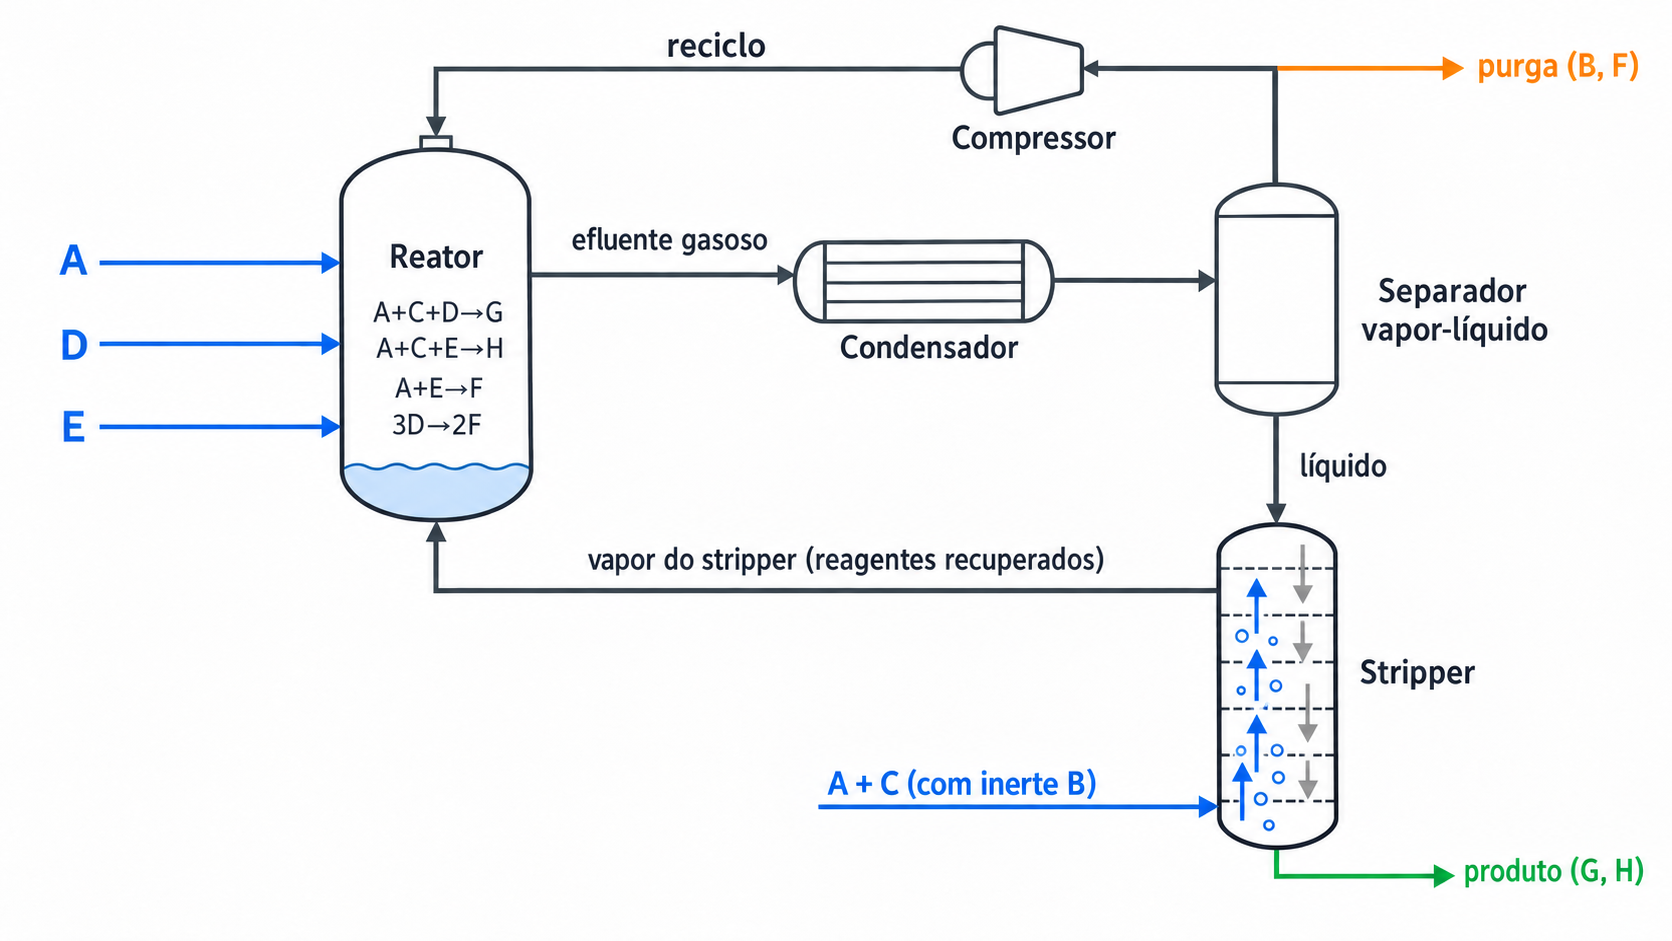
\includegraphics[width=0.92\textwidth]{imagens/tep-fluxograma.png}
	\fonte{Elaborado pelo autor, com base em \citeonline{DOWNS1993}.}
	\label{fig:tep_flowsheet}
\end{figure}

O modelo tem 50 variáveis de estado, integradas numericamente. Elas representam os inventários dos componentes e as energias no reator, no separador, no \textit{stripper} e nos demais volumes do processo. O código original foi escrito em FORTRAN.

O modelo expõe 41 variáveis medidas (XMEAS$_1$ a XMEAS$_{41}$) e 12 variáveis manipuladas (XMV$_1$ a XMV$_{12}$). As variáveis medidas incluem vazões, composições, temperaturas, pressões e níveis. As variáveis manipuladas incluem vazões de alimentação, posições de válvula (reciclo, purga, vapor do \textit{stripper}), vazões de água de resfriamento e a velocidade do agitador. No ponto de operação nominal (Modo~1), a pressão do reator é de 2705~kPa, a temperatura do reator é de 120,4~°C e a razão mássica G/H é de 50/50 \cite{DOWNS1993}.

O modelo inclui 20 distúrbios (IDV$_1$ a IDV$_{20}$). Entre eles estão mudanças na composição e na temperatura das alimentações, mudanças na temperatura da água de resfriamento, perda da alimentação de A, redução da disponibilidade de C, deriva lenta da cinética de reação e válvulas travando. Cada distúrbio é do tipo degrau, variação aleatória, deriva lenta, travamento ou desconhecido. O artigo também define limites de parada (\textit{shutdown limits}), parte da estratégia de intertravamento do processo: se uma variável ultrapassa esses limites, a planta é desligada. São exemplos a pressão do reator acima de 3000~kPa e o volume de líquido no reator fora da faixa de 2,0 a 24,0~m³. Neste trabalho, esse desligamento é chamado de ISD (\textit{Interlock Shutdown}), nome usado na implementação. A Figura~\ref{fig:tep_blocos} resume as entradas e saídas do modelo.

\begin{figure}[htbp]
	\centering
	\caption{Entradas e saídas do modelo do Processo Tennessee Eastman.}
	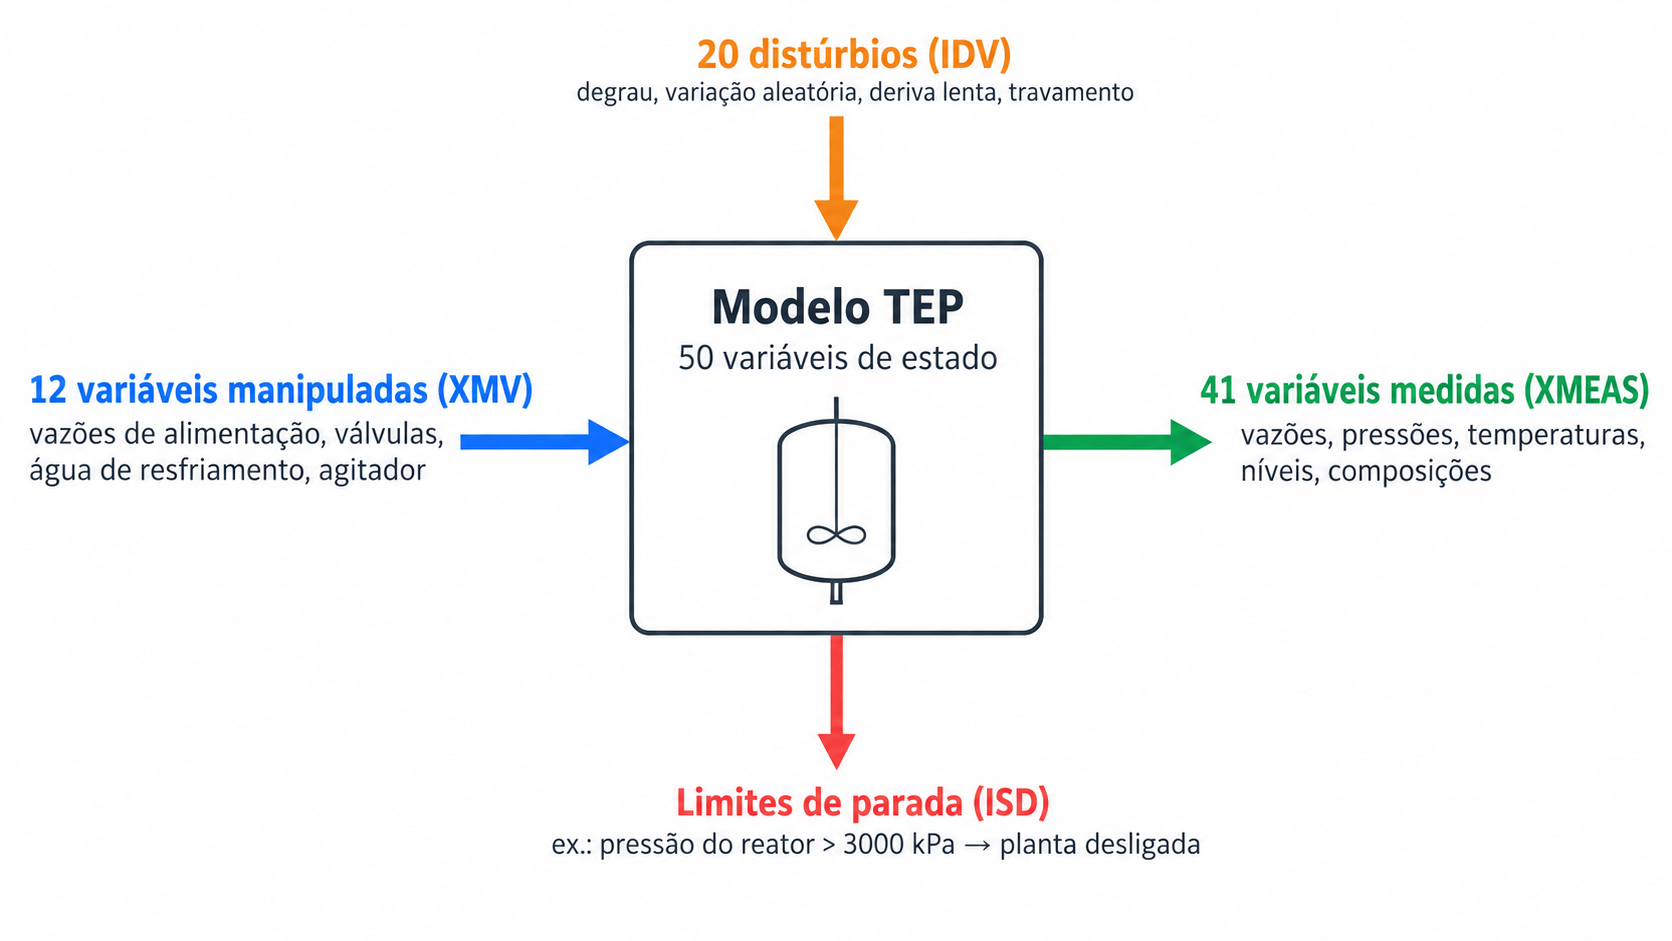
\includegraphics[width=0.85\textwidth]{imagens/tep-modelo-blocos.png}
	\fonte{Elaborado pelo autor, com base em \citeonline{DOWNS1993}.}
	\label{fig:tep_blocos}
\end{figure}

O TEP é um bom \textit{benchmark} porque reúne não-linearidades, acoplamento entre malhas, reciclo e distúrbios de naturezas diferentes. Por isso, este trabalho o usa para testar uma arquitetura de controle supervisório que depende de comunicação distribuída e de coordenação entre componentes diferentes. Essa aplicação é uma escolha deste trabalho, e não algo proposto por Downs e Vogel.

% -------------------------------------------------------------------------

\section{Controle Plant-Wide}
\label{sec:plantwide}

O TEP mostra o que a planta tem, mas não diz como organizar o controle dela. Na verdade, o problema proposto sequer seria resolvido com uma simples sintonia de malha, é preciso decidir quais variáveis controlar, quais manipular, como ligar umas às outras e como coordenar a operação da planta inteira. Essas decisões são de projeto da estrutura de controle, e é delas que trata o controle \textit{plant-wide}.

Essas decisões dependem do que se espera da planta. Downs e Vogel definem seis modos de operação, cada um com uma razão G/H e uma taxa de produção \cite{DOWNS1993}. O modo diz o que a planta deve produzir, mas não diz como. Além de cumprir o modo, a planta precisa ficar dentro dos seus limites de operação e não gastar mais do que o necessário.\footnote{Mais adiante, veremos que, neste trabalho, esse conjunto de modo, limites de operação e custo será chamado de \textbf{Política da Planta}.} Depois de atender a tudo isso, sobra pouca liberdade para o controle, e a pergunta passa a ser como usar bem essa liberdade.

Em uma planta contínua, cada malha regulatória cuida de uma variável do seu equipamento. Isso funciona bem: com malhas locais em cascata, é possível controlar plantas grandes sem precisar de um modelo detalhado \cite{Larsson2000}. O problema é que nenhuma dessas malhas olha para a planta inteira. Larsson e Skogestad lembram que os equipamentos estão ligados uns aos outros, e um acaba agindo como distúrbio para o seguinte. Em regime, por exemplo, todos precisam processar a mesma vazão. Com reciclo e integração de calor, como no TEP, essas interações aumentam. Por isso, além das malhas locais, é preciso pensar o controle da planta como um todo \cite{Larsson2000}.

Isso vale até para dizer se uma malha está boa ou não. Em um caso relatado no CERN, uma malha de nível regulava bem, mas fazia o atuador oscilar muito, o que poderia trazer problemas para a operação ao longo do tempo. Os operadores mudaram a sintonia: o atuador ficou mais suave, mas o nível passou a oscilar mais, e a ferramenta de monitoramento passou a classificar a malha como mal sintonizada.\footnote{Por ora, omitimos o método que a ferramenta usa para concluir que a sintonia piorou. Ele será apresentado na Seção~\ref{sec:diagnostico}.} Mesmo assim, a equipe preferiu a nova sintonia, porque o nível podia oscilar um pouco desde que ficasse acima de 50\%, e a oscilação do atuador não \cite{Bradu2018}. Olhando só para a malha, ela piorou; olhando para a operação, ela melhorou.

O Modo~1 ajuda a ver o que isso significa na prática. Nele, a planta deve produzir 7038~kg/h de G e 7038~kg/h de H, ou seja, uma razão G/H de 50/50 \cite{DOWNS1993}. O artigo também define limites de operação, como pressão do reator abaixo de 2895~kPa, temperatura do reator abaixo de 150~°C e faixas para os níveis do reator, do separador e do \textit{stripper}. O modo e os limites funcionam como condições de contorno: dizem aonde a planta precisa chegar e por onde ela não pode passar, mas não dizem por qual caminho.

\begin{figure}[htbp]
	\centering
	\caption{Variáveis manipuladas ocupadas pelo modo e pela estabilização dos níveis no Modo~1.}
	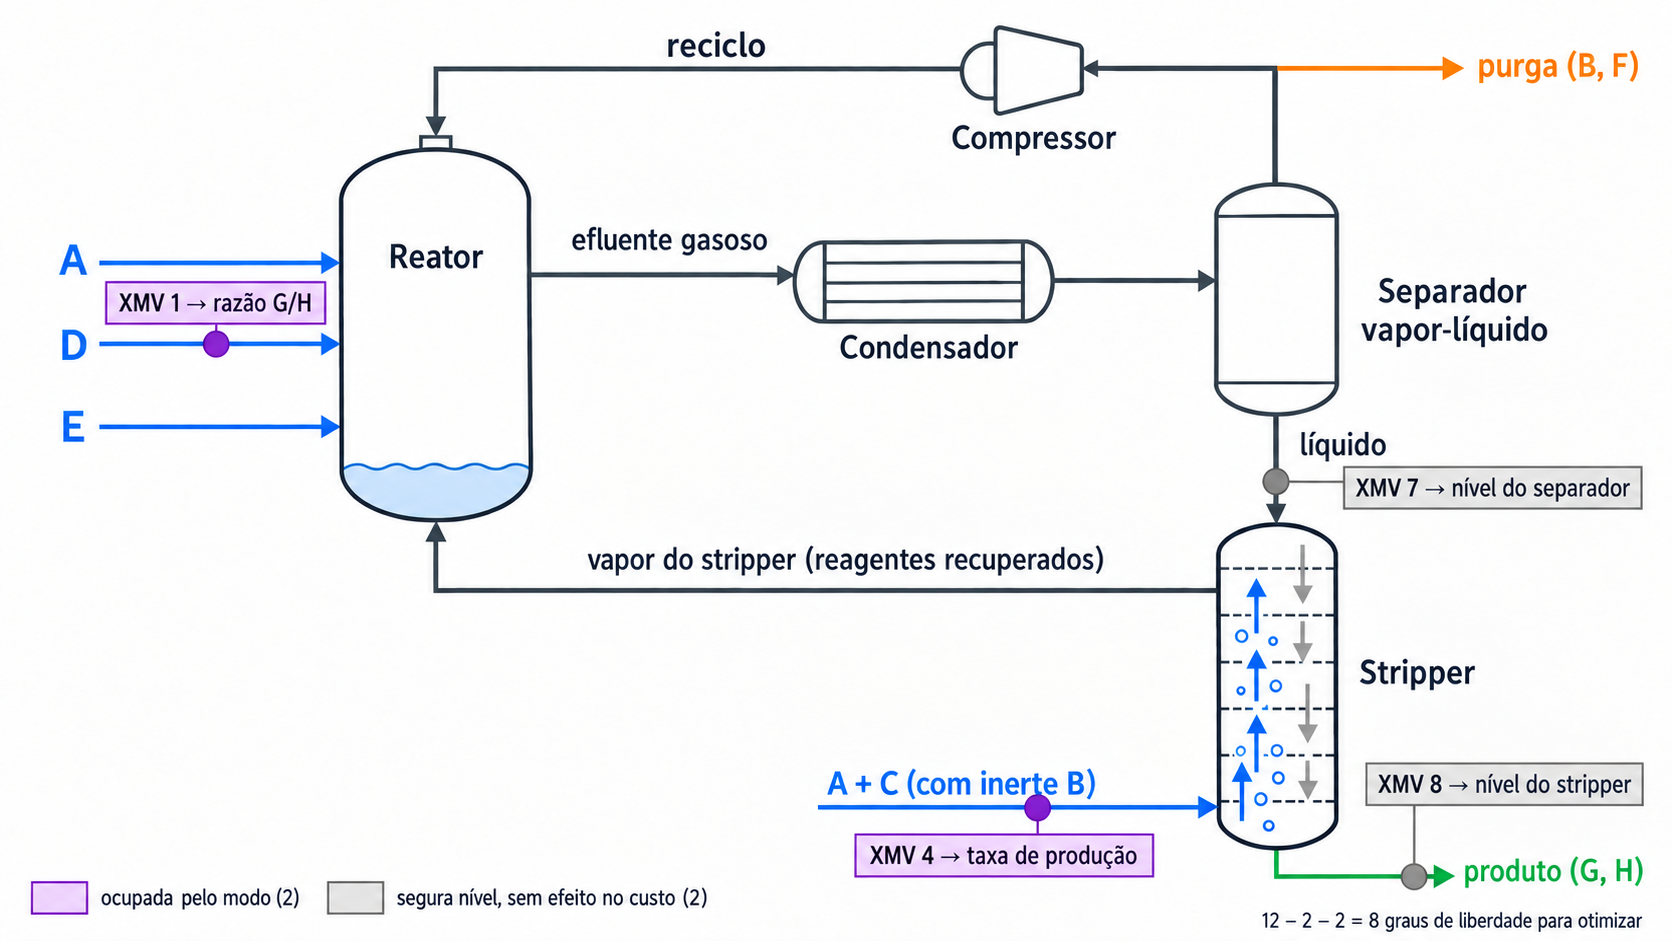
\includegraphics[width=0.95\textwidth]{imagens/tep-variaveis-ocupadas.png}
	\fonte{Elaborado pelo autor, com base em \citeonline{Larsson2001}.}
	\label{fig:tep_ocupadas}
\end{figure}

Cumprir o modo já ocupa parte das escolhas. Das 12 variáveis manipuladas (XMV$_1$ a XMV$_{12}$), cada uma é uma escolha independente. Uma delas precisa fixar a taxa de produção, e outra precisa fixar a razão G/H. No pareamento proposto por \citeonline{Larsson2001}, essas duas tarefas ficam com a alimentação de A e C (XMV$_4$) e com a alimentação de D (XMV$_1$).

Na Figura~\ref{fig:tep_ocupadas}, as duas variáveis em cinza seguram os níveis do separador e do \textit{stripper}. Esses níveis precisam de uma malha de controle para a planta ficar estável, mas o valor deles não muda o custo em regime \cite{Larsson2001}. Descontadas as duas variáveis em roxo e as duas em cinza, sobram $12 - 2 - 2 = 8$ graus de liberdade em regime estacionário; outro pareamento trocaria as válvulas, mas não a conta \cite{Larsson2001}. Há mais de uma forma de usar esses oito graus de liberdade para cumprir o Modo~1, e elas não custam o mesmo \cite{DOWNS1993}. Para escolher entre elas, é preciso um critério de custo.

\subsection{Função de custo como ponto de partida}
\label{subsec:custo}

Antes de escolher a estrutura de controle, \citeonline{Skogestad2004} estabelece um
pré-requisito frequentemente negligenciado: a definição explícita dos objetivos operacionais. Sem um
critério de desempenho claro, a escolha entre controlar temperatura do reator, vazão de reciclo ou
composição na purga torna-se arbitrária — uma questão de opinião ou convenção, não de análise.
Idealmente, esses objetivos devem ser combinados em uma função de custo escalar $J$ a ser minimizada:

\begin{quote}
	\textit{``The operational objectives must be clearly defined before attempting to design a control
		system. Although this seems obvious, this step is frequently overlooked. Preferably, the operational
		objectives should be combined into a scalar cost function J to be minimized. In many cases, J may be
		simply selected as the operational cost.''} \cite{Skogestad2004}
\end{quote}

O artigo original de \citeonline{DOWNS1993} fornece exatamente essa função de custo para o TEP,
expressa em termos de custos operacionais com coeficientes numéricos específicos (Tabela~9 do artigo
original). De forma conceitual, a lógica econômica dessa função pode ser entendida como a soma
ponderada de cinco componentes de perda: (a)~perda de reagentes não convertidos na corrente de
purga; (b)~perda de matérias-primas na corrente de produto; (c)~formação do subproduto F, que
representa reagentes consumidos sem retorno econômico; (d)~trabalho do compressor; e (e)~consumo de
vapor. A representação abaixo sintetiza essa estrutura — mas não deve ser entendida como transcrição
literal dos termos da Tabela~9:

\begin{equation}
	J = c_{\mathrm{purga}} \cdot \dot{m}_{\mathrm{purga}}
	+ c_{\mathrm{prod}} \cdot \dot{m}_{\mathrm{MP,prod}}
	+ c_F \cdot \dot{m}_F
	+ c_{\mathrm{comp}} \cdot W_{\mathrm{comp}}
	+ c_{\mathrm{vapor}} \cdot \dot{Q}_{\mathrm{vapor}}
	\label{eq:tep_cost}
\end{equation}

\noindent onde cada termo representa, respectivamente: custo das matérias-primas perdidas na purga,
custo das matérias-primas que saem com o produto, custo econômico atribuído à formação de F, custo
do trabalho de compressão e custo do vapor. O sinal de $J$ está formulado como custo (negativo de
lucro), de modo que minimizar $J$ corresponde a maximizar a eficiência operacional \cite{DOWNS1993}.

Cabe destacar que $J$ não é uma equação natural da planta, derivável de primeiros princípios como
as Equações~\ref{eq:rx1}--\ref{eq:rx4}: ela é uma escolha de formulação. \citeonline{Williams2013}
observa que toda formulação de programação matemática compartilha a característica de envolver
otimização — deseja-se maximizar ou minimizar uma quantidade, denominada função objetivo — e que,
dado um mesmo conjunto de restrições, objetivos distintos conduzem a soluções ótimas distintas.
O autor cataloga exemplos típicos de objetivo (maximizar lucro, minimizar custo, maximizar
utilidade, maximizar valor presente líquido, maximizar robustez) que ilustram o mesmo ponto
explorado por \citeonline{Skogestad2004} para o TEP: a função de custo traduz uma política
operacional escolhida pelo projetista, não uma propriedade física da planta.

Com $J$ definida, dá para dizer o que fazer com os oito graus de liberdade. Minimizando $J$ no Modo~1, cinco deles levam variáveis ao limite: pressão do reator no máximo, nível do reator no mínimo, válvula de reciclo do compressor fechada, válvula de vapor do \textit{stripper} fechada e agitador no máximo. Sobram três graus de liberdade livres \cite{Larsson2001}. A Tabela~\ref{tab:graus_liberdade} mostra o uso das 12 variáveis manipuladas, a Figura~\ref{fig:graus_liberdade_tep} resume a conta e a Figura~\ref{fig:tep_modo1} mostra essas variáveis na planta. Usar um grau de liberdade livre significa escolher uma variável e mantê-la constante com uma malha de controle. A combinação da tabela (temperatura do reator, \% de C na purga e vazão de reciclo) é a de menor perda entre as que \citeonline{Larsson2001} consideram aceitáveis.

\begin{figure}[htbp]
	\centering
	\caption{Meta, variáveis no limite e uma escolha para os graus de liberdade livres do TEP no Modo~1.}
	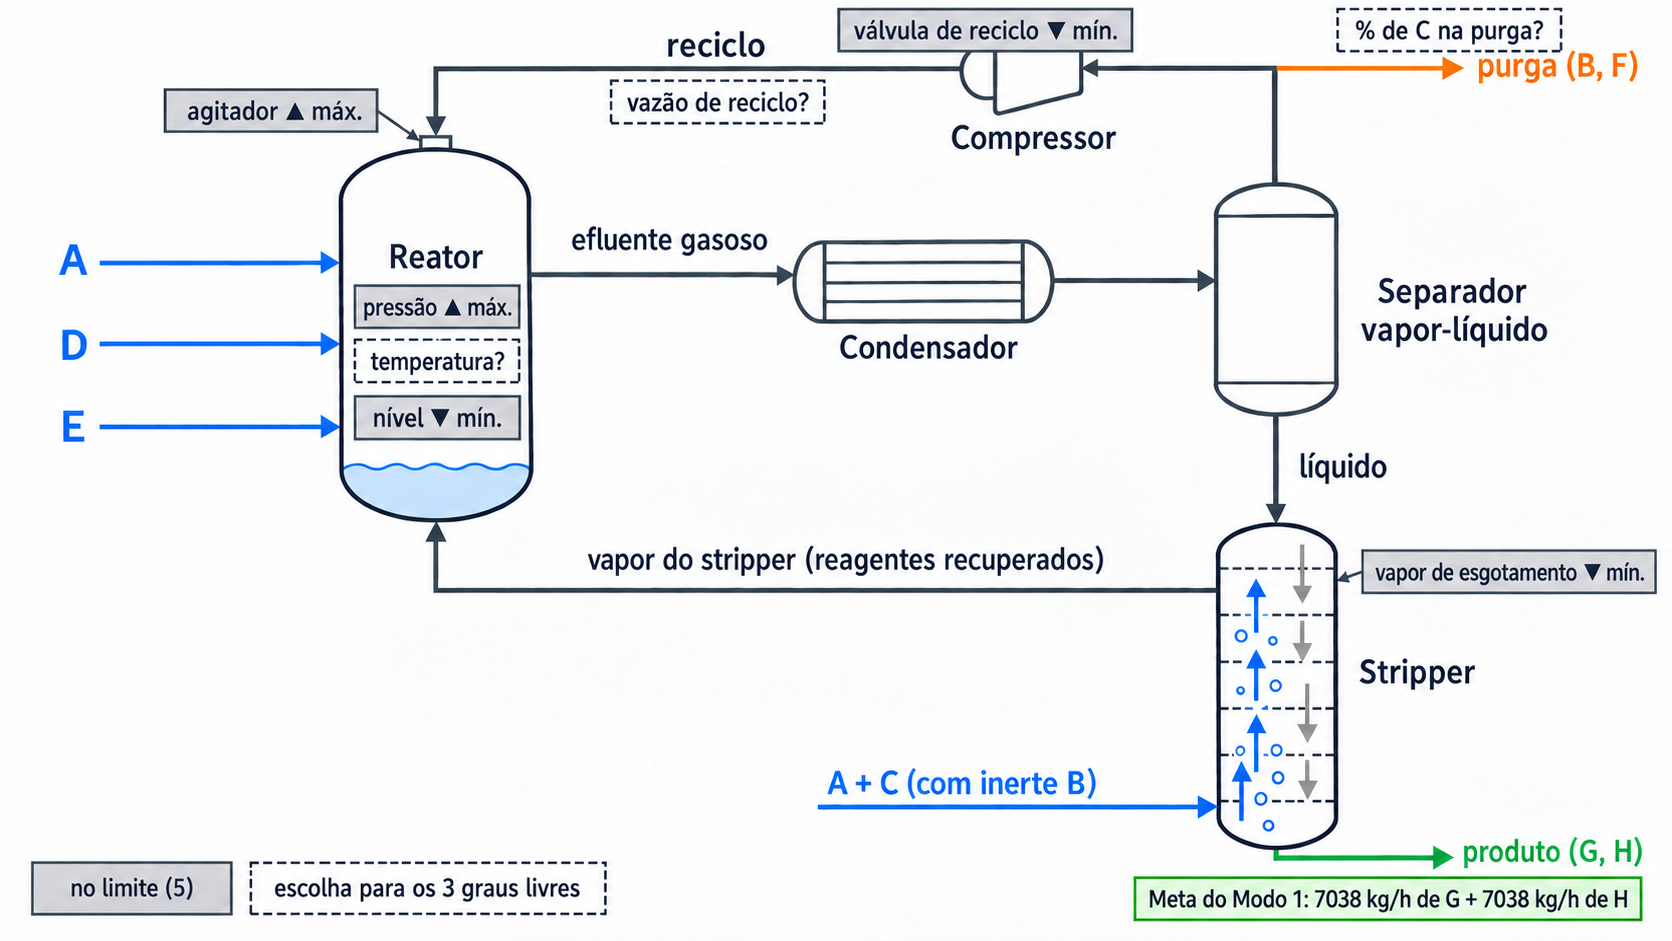
\includegraphics[width=0.95\textwidth]{imagens/tep-modo1-graus-liberdade.png}
	\fonte{Elaborado pelo autor, com base em \citeonline{DOWNS1993} e \citeonline{Larsson2001}.}
	\label{fig:tep_modo1}
\end{figure}

\begin{table}[htbp]
	\centering
	\caption{Uso dos 12 graus de liberdade do TEP no ótimo do Modo~1.}
	\label{tab:graus_liberdade}
	\small
	\begin{tabular}{|>{\raggedright\arraybackslash}p{2.9cm}|c|>{\raggedright\arraybackslash}p{3.7cm}|>{\raggedright\arraybackslash}p{3.8cm}|>{\raggedright\arraybackslash}p{2.9cm}|}
		\hline
		\textbf{Grupo} & \textbf{XMV} & \textbf{Variável manipulada} & \textbf{Variável controlada} & \textbf{No Modo~1} \\
		\hline
		\multirow{2}{2.9cm}{\raggedright Nível sem efeito no custo ($-2$)}
		  & 7  & líquido do separador          & nível do separador         & qualquer \\
		  & 8  & produto do \textit{stripper}  & nível do \textit{stripper} & qualquer \\
		\hline
		\multirow{2}{2.9cm}{\raggedright Exigido pelo modo ($-2$)}
		  & 4  & alimentação A + C             & taxa de produção           & 7038~kg/h de G e de H \\
		  & 1  & alimentação de D              & razão G/H                  & 50/50 \\
		\hline
		\multirow{5}{2.9cm}{\raggedright No limite (5)}
		  & 5  & válvula de reciclo            & a própria válvula          & fechada \\
		  & 9  & vapor do \textit{stripper}    & a própria válvula          & fechada \\
		  & 12 & agitador                      & a própria velocidade       & máxima \\
		  & 2  & alimentação de E              & nível do reator            & mínimo \\
		  & 6  & válvula de purga              & pressão do reator          & máxima \\
		\hline
		\multirow{3}{2.9cm}{\raggedright Livre (3)}
		  & 10 & resfriamento do reator        & temperatura do reator      & valor ótimo \\
		  & 3  & alimentação de A              & \% de C na purga           & valor ótimo \\
		  & 11 & resfriamento do condensador   & vazão de reciclo           & valor ótimo \\
		\hline
	\end{tabular}
	\fonte{Elaborado pelo autor, com base nas Tabelas~1 e 5 de \citeonline{Larsson2001}.}
\end{table}

A existência dessa função de custo transforma a escolha das variáveis controladas em uma pergunta técnica: a melhor seleção de variáveis controladas é aquela que, sob incerteza de perturbações
e ruído, mantém $J$ mais próximo do seu valor ótimo $J^*$.

\subsection{Hierarquia de controle e escala de tempo}

\citeonline{Skogestad2004} propõe organizar a resposta a essas perguntas em uma hierarquia de
camadas separadas por escala de tempo:

\begin{enumerate}
	\item \textbf{Controle regulatório}: malhas PID locais que estabilizam variáveis de processo em
	      torno de um ponto de operação. Esse nível opera em escala de segundos a minutos e não possui
	      visão global da planta.
	\item \textbf{Controle supervisório}: coordenação das malhas regulatórias via ajuste de setpoints
	      e ativação/desativação de malhas, operando em escala de minutos a horas. Esse é o nível que
	      reage a perturbações que transcendem os limites de uma única malha local.
	\item \textbf{Otimização em tempo real} (\textit{Real-Time Optimization} --- RTO): recálculo dos
	      setpoints ótimos das variáveis primárias com base nas condições econômicas vigentes e nas
	      restrições ativas, operando em escala de horas a dias.
\end{enumerate}

A separação em camadas é justificada não apenas pela diferença de escala de tempo, mas pela
diferença de informação disponível em cada nível. A camada regulatória opera com medições locais e
sem modelo da planta inteira. A camada supervisória opera sobre os setpoints das malhas regulatórias,
sem necessidade de acessar diretamente as válvulas. A RTO, por sua vez, resolve um problema de
otimização estacionária para determinar os setpoints ótimos que a camada supervisória deve perseguir
\cite{Skogestad2004}.

\begin{figure}[htbp]
	\centering
	\missingfigure[figwidth=0.80\textwidth]{Hierarquia de controle plant-wide de Skogestad (3 camadas verticais): base = controle regulatório (malhas PID, escala de segundos a minutos); meio = controle supervisório (ajuste de setpoints e modos, escala de minutos a horas); topo = otimização em tempo real --- RTO (recálculo de setpoints ótimos via minimização de $J$, escala de horas a dias). Setas descendentes indicam setpoints; setas ascendentes indicam estados e medições. Adaptado de \citeauthor{Skogestad2004} (\citeyear{Skogestad2004}).}
	\caption{Hierarquia de controle plant-wide: regulatório, supervisório e otimização em tempo real.}
	\label{fig:plantwide_hierarchy}
\end{figure}

\subsection{Controle self-optimizing e a perda econômica}

O conceito central que conecta a função de custo $J$ à estrutura de controle é o de
\textbf{controle self-optimizing}: escolher variáveis controladas $c$ tais que, mantidas em setpoint
fixo, levem automaticamente aos ajustes ótimos das variáveis manipuladas quando ocorrem perturbações
--- sem necessidade de reotimização explícita \cite{Skogestad2004}. Para quantificar quando uma
escolha de $c$ é suficientemente boa, define-se a \textbf{perda econômica} $L$:

\begin{equation}
	L = J(u, d) - J^*(d)
	\label{eq:loss}
\end{equation}

\noindent onde $J(u,d)$ é o valor real da função de custo quando a política de setpoint fixo é
aplicada sob perturbação $d$, e $J^*(d)$ é o valor ótimo que seria atingido com reotimização
completa. O controle self-optimizing é alcançado quando existe uma política de setpoint constante
que resulta em perda $L$ aceitável para o espectro esperado de perturbações \cite{Skogestad2004}.

A implicação prática é significativa: se as variáveis controladas forem bem escolhidas, o supervisor
não precisa resolver um problema de otimização a cada perturbação --- basta regular $c$ no setpoint.
A escolha errada das variáveis controladas, por outro lado, pode resultar em perda econômica elevada
mesmo que todas as malhas estejam corretamente sintonizadas.

\subsection{Aplicação ao TEP: análise de graus de liberdade}

\citeonline{Larsson2001} aplicam essa metodologia ao TEP. Partem dos 8 graus de liberdade em regime estacionário e das 5 restrições ativas no Modo~1, vistos na Seção~\ref{subsec:custo}, e buscam variáveis \textit{self-optimizing} para os 3 graus de liberdade que sobram.

Os autores comparam as alternativas pela perda $L$, calculada com a função de custo de \citeonline{DOWNS1993}. Quatro combinações ficam abaixo da perda que eles consideram aceitável. As duas melhores são a temperatura do reator (XMEAS$_9$), a composição de C na purga e a vazão de reciclo (XMEAS$_5$) ou o trabalho do compressor (XMEAS$_{20}$). Controlar a composição do inerte B, uma sugestão comum, foi uma escolha ruim: com distúrbios ou erros de implementação, a planta pode chegar a um ponto de operação inviável \cite{Larsson2001}.

Essa análise revela a função concreta que uma camada supervisória deve exercer no TEP: não apenas
estabilizar a planta, mas garantir que as variáveis primárias $c$ --- aquelas identificadas como
self-optimizing --- permaneçam próximas de seus setpoints ótimos frente às perturbações IDV.
Qualquer arquitetura supervisória proposta pode ser avaliada, em última instância, pelo valor de $L$
que produz em simulação.

A hierarquia de Skogestad fornece o enquadramento teórico para a separação de responsabilidades na
arquitetura proposta neste trabalho: a camada regulatória é implementada pelo conjunto de
controladores PID do \texttt{ControllerBank}; a camada supervisória é o objeto de investigação
central deste trabalho --- responsável por coordenar setpoints, modos e condições observadas das
malhas regulatórias frente a perturbações e transições operacionais. A camada de otimização em tempo
real, que determinaria os setpoints ótimos de $c$ via minimização de $J$, fica fora do escopo deste
trabalho e constitui extensão natural. O TEP, com sua função de custo explícita e seus 41~XMEAS e
12~XMV, é um ambiente adequado para avaliar se um supervisor consegue manter a planta próxima do
ótimo operacional sem requerer reotimização a cada perturbação.

A camada de RTO, embora fora do escopo de implementação, é explorada preliminarmente no
Apêndice~\ref{apendice:otimizacao}, onde a função de custo $J$ é estendida para incorporar outras
dimensões de desempenho operacional -- operação, qualidade, energia, risco, manutenção e produção
perdida -- e diferentes algoritmos de otimização são avaliados como candidatos a traduzir essas
funções objetivo em políticas supervisórias concretas para o Kubernetes.

% -------------------------------------------------------------------------

\section{Cloud-Native como Paradigma de Orquestração Industrial}
\label{sec:cloudnative}

A hierarquia de controle plant-wide estabelece a existência e a função de uma camada supervisória: ela deve observar o estado de múltiplos controladores distribuídos pela planta, propagar decisões de coordenação --- setpoints, modos, políticas --- e reagir a perturbações sem executar diretamente as malhas regulatórias. Isso coloca uma questão de implementação que o referencial de controle de processos não responde: qual paradigma tecnológico suporta construir um sistema distribuído capaz de observar componentes heterogêneos, manter um estado operacional desejado e tomar ações corretivas de forma contínua e autônoma? É a esse problema que o paradigma cloud-native se dirige.

O termo \textit{cloud-native} designa uma abordagem de desenvolvimento e operação de sistemas distribuídos que explora recursos típicos da computação em nuvem --- conteinerização, microsserviços, orquestração automática de containers, DevOps e pipelines de entrega contínua \cite{Shuiguang2023}. Conforme \citeonline{Shuiguang2023}, uma aplicação cloud-native pode ser entendida como um sistema distribuído, elástico e escalável horizontalmente, composto por microsserviços inter-relacionados empacotados em containers leves e orquestrados sobre múltiplos servidores. Nesse paradigma, a orquestração é descrita pelos autores como a configuração, o gerenciamento e a coordenação automatizados do ciclo de vida dos containers --- provisionamento, implantação, agendamento, escalonamento, configuração de rede e balanceamento de carga --- de modo a manter as funcionalidades da aplicação elásticas e disponíveis. O Kubernetes, originado do gerenciador de clusters Borg do Google, é descrito pelos mesmos autores como o software open-source de orquestração de containers mais popular e como um padrão de fato amplamente adotado pela indústria.

\citeonline{Burns2016} documentam a evolução dos sistemas de orquestração do Google --- Borg, Omega e Kubernetes --- e mostram que a força do Kubernetes está na combinação de uma API uniforme, objetos extensíveis e separação explícita entre estado desejado e estado observado. Cada recurso Kubernetes é representado como um objeto com dois campos centrais: \textit{Spec}, que descreve o estado desejado, e \textit{Status}, que registra o estado observado em tempo de execução. Sobre essa estrutura operam controladores de reconciliação (\textit{reconciliation controller loops}) que comparam continuamente o estado desejado ao estado observado e executam ações para convergir o segundo em direção ao primeiro \cite{Burns2016}. Os autores destacam ainda que a conteinerização muda o paradigma operacional dos data centers --- de uma perspectiva orientada a máquinas para uma perspectiva orientada a aplicações, na qual gerenciar containers significa gerenciar aplicações, não servidores. Essa combinação de API uniforme, objetos Spec/Status, controladores de reconciliação e extensibilidade torna o Kubernetes uma plataforma de operação declarativa para sistemas distribuídos complexos. No ecossistema Kubernetes, essa lógica declarativa pode ser estendida pelo \textit{Operator Pattern}, no qual controladores específicos de domínio observam recursos customizados e executam ações de reconciliação sobre aplicações ou sistemas externos ao cluster.

\begin{figure}[htbp]
	\centering
	\missingfigure[figwidth=0.85\textwidth]{Loop de reconciliação do Kubernetes: (1) objeto com \textit{Spec} (estado desejado declarado pelo operador) e \textit{Status} (estado observado em tempo real); (2) controlador de reconciliação compara Spec e Status; (3) se divergentes, aciona ação corretiva (e.g., reiniciar pod, ajustar réplicas, atualizar rota); (4) sistema converge e Status se aproxima de Spec. Pode incluir exemplo industrial análogo: \textit{Spec} = modo operacional desejado da planta; \textit{Status} = condição observada das malhas; ação = ajuste de setpoint ou reconfiguração. Baseado em \citeauthor{Burns2016} (\citeyear{Burns2016}).}
	\caption{Loop de reconciliação Spec/Status do Kubernetes e sua analogia com supervisão industrial.}
	\label{fig:k8s_reconciliation}
\end{figure}

A relevância desse paradigma para sistemas industriais não está em substituir controladores regulatórios ou malhas de tempo real, mas em oferecer uma forma de organizar camadas superiores de operação: implantação e ciclo de vida de serviços, supervisão de componentes distribuídos, observabilidade, tolerância a falhas, aplicação de políticas e coordenação de estados operacionais. Nesse enquadramento, cloud-native e Kubernetes são considerados como referências para a camada supervisória e informacional do sistema, preservando a distinção entre controle regulatório da planta e orquestração da infraestrutura de software.

\subsection{Precedentes Industriais}

Trabalhos recentes indicam que essa aproximação entre infraestrutura cloud-native e automação industrial já é objeto de pesquisa. \citeonline{Johansson2022} investigam o uso de Kubernetes para orquestrar nós controladores distribuídos virtualizados (\textit{Virtual Distributed Control Nodes}, VDCNs) em cenários de alta disponibilidade. A lógica de controle permanece no interior dos VDCNs; o Kubernetes atua como camada de orquestração, executando o agendamento situacional dos containers, gerenciando os laços de reconciliação que empurram o estado atual em direção ao estado desejado, e atualizando as rotas de comunicação conforme o estado da aplicação --- determinando qual instância VDCN recebe comandos OPC~UA e, portanto, qual controlador participa ativamente da operação. Diante de falhas de nó, o Kubernetes detecta o evento, reimplanta o VDCN afetado e, no caso redundante, promove o backup a primário enquanto cria uma nova instância de backup \cite{Johansson2022}. Esse resultado é relevante porque mostra um precedente em que o Kubernetes é usado não apenas como infraestrutura genérica, mas como camada responsável por recompor componentes de controle industrial diante de falhas, com efeito direto sobre a continuidade operacional do sistema.

\citeonline{Mellado2022} propõem o \textbf{IoT-PLC}, uma arquitetura baseada em containers para CLPs orientados à Indústria~4.0, na qual cada funcionalidade --- controle regulatório, armazenamento de dados de campo, interfaces sem fio --- é encapsulada em um container separado. O IoT-PLC é posicionado como nó de fog computing, mantendo a execução próxima à planta enquanto permite gerenciamento direto a partir da nuvem, reconfiguração a quente de malhas de controle e ajuste de recursos computacionais por container sem interromper o processo. O artigo utiliza também um \textit{modelo de dispositivo virtual} que abstrai a interface do controlador para camadas superiores. Embora não constitua uma implementação baseada em Kubernetes, o IoT-PLC é relevante como antecedente conceitual: ele mostra que a literatura industrial já considera plausível decompor funções de CLP em componentes conteinerizados, reconfiguráveis e gerenciáveis externamente, e representar entidades físicas por abstrações digitais acessíveis a camadas superiores --- uma preocupação compatível com a lógica de recursos declarativos usada em arquiteturas cloud-native.

Em conjunto, esses trabalhos indicam uma convergência entre práticas cloud-native e sistemas industriais, mas também delimitam seu escopo. Uma limitação importante é que o Kubernetes não foi projetado para controle determinístico de tempo real: seus mecanismos de agendamento, reinicialização e redistribuição de cargas são adequados para disponibilidade e operação de aplicações distribuídas, mas não garantem, por si só, tempos de resposta compatíveis com malhas regulatórias industriais. A contribuição mais defensável dos princípios cloud-native está na camada supervisória --- observação de componentes distribuídos, manutenção de configurações desejadas, recomposição de serviços após falhas e disponibilização de abstrações operacionais para camadas superiores ---, sem substituir a execução determinística de controladores de baixo nível. A integração com ativos industriais pressupõe ainda uma camada de comunicação capaz de representar medições, comandos e estados de equipamentos de forma estruturada; protocolos como OPC~UA são relevantes nesse ponto, funcionando como possível interface entre a camada de orquestração e os dispositivos de automação.

% -------------------------------------------------------------------------

\section{Diagnóstico de Qualidade de Malhas}
\label{sec:diagnostico}

O paradigma cloud-native oferece a infraestrutura para observar componentes distribuídos, manter estados desejados e acionar ações corretivas. O problema é que o Kubernetes --- ou qualquer camada supervisória de software --- opera sobre abstrações que nada têm a ver com o vocabulário da planta: ele conhece pods, serviços, configurações e rotas, não variáveis de processo, setpoints ou oscilações em malhas PID. Para que um orquestrador possa tomar decisões sobre o estado operacional de uma planta, é necessário um passo anterior: sair dos sinais brutos gerados pelos controladores e produzir estados reconhecíveis em nível de supervisão. Isso exige uma camada analítica que saiba interpretar séries temporais de processo e traduzi-las em condições que o supervisor possa consumir --- malha saudável, malha degradada, atuador saturado, comportamento o'scilatório. É dessa tradução que trata o diagnóstico de qualidade de malhas.

A qualidade de uma malha de controle não é binária: um controlador pode estar em modo automático e ainda assim apresentar desempenho degradado. Malhas excessivamente agressivas podem induzir oscilações e desgaste de atuadores; malhas conservadoras demais respondem lentamente e permitem a propagação de distúrbios; e restrições de atuador, ruído de medição ou perturbações externas podem comprometer o comportamento da malha sem necessariamente acionar alarmes discretos. Em plantas com centenas ou milhares de controladores, a identificação manual de condições degradadas torna-se impraticável, motivando técnicas de \textit{control loop performance monitoring} (CLPM). O objetivo do CLPM não é controlar melhor diretamente, mas transformar históricos de sinais da malha --- setpoint, variável medida e saída do controlador --- em indicadores de desempenho que permitam priorizar quais malhas exigem análise especializada \cite{Bradu2018}.

\subsection{Benchmark de Variância Mínima e o Índice de Harris}

O trabalho de \citeonline{Harris1989} tornou-se um marco clássico na avaliação quantitativa de desempenho de malhas fechadas ao propor um benchmark baseado em controle de variância mínima. A ideia central é que, para processos representáveis por funções de transferência lineares sujeitos a perturbações aditivas, existe um limite inferior teórico para a variância da variável controlada: a variância que seria obtida por um controlador de variância mínima (MVC), dado o atraso discreto inerente ao processo. A principal contribuição de Harris é que esse limite pode ser estimado a partir de dados rotineiros de operação em malha fechada --- sem experimentos de identificação ou conhecimento completo do modelo --- bastando conhecer o atraso discreto efetivo $f$ (número de períodos de amostragem entre a ação de controle e seu efeito mensurável na saída).

A estimativa de $\sigma^2_{\text{mv}}$ é obtida ajustando-se um modelo univariado de séries temporais à variável controlada em malha fechada e extraindo a variância do erro de previsão $f+1$ passos à frente. Essa variância corresponde à parcela da saída que não pode ser removida por \textit{feedback} antes que o efeito do atraso se manifeste, e está associada aos primeiros coeficientes da representação de médias móveis da dinâmica de perturbação \cite{Harris1989}. Uma propriedade diagnóstica importante decorre diretamente da teoria: sob controle de variância mínima, a autocorrelação da variável controlada é nula além do lag $f$. Portanto, autocorrelação significativa para lags maiores que $f$ indica que o controlador não está extraindo todo o desempenho possível com a estrutura de controle vigente.

Em formulações de CLPM posteriores ao trabalho original, o desempenho é expresso como:

\begin{equation}
	\eta = \frac{\sigma^2_{\text{mv}}}{\sigma^2_y}
	\label{eq:harris_index}
\end{equation}

\noindent Valores próximos de 1 indicam operação próxima ao benchmark de variância mínima; valores baixos indicam variância observada substancialmente maior do que o limite alcançável. Deve-se observar que o índice não identifica a causa da degradação: um baixo $\eta$ pode decorrer de má sintonia, mas também de atraso excessivo, saturação de atuador, ruído de medição, ausência de ação feedforward ou perturbação não medida. Quando $\eta$ está próximo de 1, mas a variância absoluta ainda é elevada, a causa é estrutural --- e reduções adicionais de variância só são alcançáveis por modificações no processo, como redução de atraso, troca de variável manipulada ou adição de feedforward \cite{Harris1989}.

\subsection{Índice de Preditividade e a Abordagem do CERN}

Embora o benchmark de Harris forneça uma referência teórica robusta, sua aplicação pressupõe hipóteses de linearidade e requer o conhecimento de $f$. Abordagens posteriores de CLPM buscaram métricas mais simples de implantar em larga escala, operando diretamente sobre históricos de malhas sem modelo físico da planta. É nesse contexto que se insere o \textit{Predictability Index} (PI) aplicado por \citeonline{Bradu2018} ao sistema criogênico do LHC, que opera milhares de malhas PID distribuídas ao longo do acelerador. Nessa escala, a inspeção manual é inviável, e o PI funciona como métrica automática de triagem.

O método prediz o erro futuro da malha a partir de seus valores passados. Para um horizonte de predição $b$ e uma ordem de modelo $m$, o erro previsto é:

\begin{equation}
	\hat{e}(t+b) = a_0 + a_1\,e(t) + a_2\,e(t-1) + \cdots + a_m\,e(t-m-1)
	\label{eq:pi_pred}
\end{equation}

A partir do resíduo de predição, calcula-se:

\begin{equation}
	\text{PI} = \frac{\sigma^2_r}{\text{mse}}
	\label{eq:pi_index}
\end{equation}

\noindent onde $\sigma^2_r$ é a variância do resíduo entre o erro medido e o erro previsto e
$\text{mse}$ é o erro quadrático médio da malha. Operacionalmente, PI baixo indica comportamento
errático ou imprevisível; PI alto indica comportamento regular compatível com o modelo adotado
\cite{Bradu2018}.

Os parâmetros do método são derivados de grandezas operacionais: intervalo de amostragem $t_s$, janela de análise $T_W$ e constante de tempo característica da malha $T$. A partir dessas grandezas, calculam-se o número de amostras da janela $n = \lceil T_W/t_s \rceil$, o horizonte de predição $b = \lceil T/t_s \rceil$ e a ordem do modelo $m = 2b$. Essa estrutura permite configurar o método por grupos de malhas, sem ajuste individual para cada controlador.

A classificação de uma malha como problemática não depende apenas do valor bruto do PI. Os autores adicionam duas condições operacionais para reduzir falsos positivos: (i)~a saída do controlador deve apresentar variação significativa ($\sigma_y > \bar{\sigma}_y$), evitando classificar como degradadas malhas saturadas, inativas ou em modo manual; e (ii)~a condição PI~$< PI_L$ deve persistir em mais de $N$ janelas dentro de um período de 24 horas, evitando que transientes breves sejam interpretados como degradação estrutural. O limiar $PI_L$ não é uma constante universal: no artigo do CERN, ele é definido empiricamente por grupos de controladores --- temperatura, pressão, vazão e nível --- com valores distintos conforme a dinâmica e os objetivos operacionais de cada grupo \cite{Bradu2018}.

Quando uma malha é declarada problemática pelo PI, o artigo classifica a causa em quatro categorias: (i)~\textit{tuning} --- o controlador precisa ser resintonizado; (ii)~\textit{process} --- o controlador não lida adequadamente com os distúrbios, inclusive por restrições mecânicas; (iii)~\textit{noise} --- a variável medida apresenta ruído excessivo para uma regulagem eficaz; e (iv)~\textit{false positive} --- os parâmetros do PI estão inadequados para aquela malha específica. PI baixo, portanto, não implica diretamente em PID mal sintonizado; a causa exige diagnóstico complementar \cite{Bradu2018}.

\begin{figure}[htbp]
	\centering
	\missingfigure[figwidth=0.90\textwidth]{Pipeline do CLPM: da esquerda para a direita --- (1) série temporal bruta da malha (setpoint, variável medida, saída do controlador); (2) cálculo de índices: Harris $\eta = \sigma^2_{\text{mv}}/\sigma^2_y$ e Predictability Index $\text{PI} = \sigma^2_r/\text{mse}$; (3) estado diagnóstico resultante (malha saudável / degradada / oscilatória / ruidosa). Pode incluir exemplo de série temporal contrastando malha saudável ($\eta \approx 1$, PI alto) com malha degradada ($\eta \ll 1$, PI baixo). Baseado em \citeauthor{Harris1989} (\citeyear{Harris1989}) e \citeauthor{Bradu2018} (\citeyear{Bradu2018}).}
	\caption{Pipeline conceitual do diagnóstico de qualidade de malhas (CLPM): de sinais brutos a estados supervisionáveis.}
	\label{fig:clpm_pipeline}
\end{figure}

\subsection{Detecção de Padrões Dinâmicos e Anomalias}

Além de índices globais de desempenho, trabalhos do mesmo grupo investigam a detecção de padrões específicos de comportamento anômalo. \citeonline{Tilaro2017} propõem um método de detecção online de oscilações em sensores e atuadores que combina análise espectral por transformada de Fourier discreta (DFT), filtro passa-faixa, detecção de cruzamentos por zero e verificação de regularidade temporal. Uma propriedade relevante do método é que oscilações podem ocorrer mesmo quando o sistema opera em estado nominal, sem acionar qualquer alarme discreto de limiar. O método formaliza o julgamento tácito do especialista --- que identificava visualmente padrões anômalos nas tendências de válvulas e medições --- em uma análise computável, produzindo condições interpretadas caracterizadas por frequência dominante, amplitude, período e índice de regularidade.

\citeonline{Tilaro2018} estendem essa direção com métodos de aprendizado de modelos sobre dados históricos de controle, explorando relações físicas e lógicas entre sinais para detectar desvios coerentes em relação ao comportamento histórico esperado. Desvios persistentes funcionam como sinais de aviso de possíveis anomalias futuras, ativando verificações por especialistas antes que falhas se manifestem.

A mesma lógica de transformar séries temporais em estados de saúde supervisionáveis estende-se ao monitoramento de condição de equipamentos. \citeonline{Lessmeier2016} demonstram que sinais de corrente elétrica de motores, disponíveis nos inversores de frequência já presentes na instalação sem necessidade de sensores adicionais, carregam informação sobre danos em mancais do sistema de acionamento. O estado relevante --- dano no mancal, sua localização e extensão --- não é medido diretamente: ele é um estado latente inferido a partir de assinaturas espectrais e estatísticas extraídas da série temporal de corrente. Esse trabalho é particularmente relevante no contexto de atuadores de processo, como bombas e compressores, cujos defeitos mecânicos incipientes podem se manifestar como degradação de desempenho de malhas de controle antes de qualquer alarme de processo --- ou seja, como uma das categorias \textit{process} do PI de \citeonline{Bradu2018}.

Em trabalho de iniciação científica desenvolvido pelo autor sob orientação do Prof.\ Dr.\ Luiz Alberto Pinto, a análise via transformada \textit{wavelet} foi investigada como extensão dessa abordagem. A decomposição \textit{wavelet} permite decompor o sinal de corrente em múltiplas escalas de frequência e tempo simultaneamente, capturando assinaturas transitórias de falha que métodos baseados exclusivamente em análise de Fourier podem deixar passar. Os resultados obtidos nessa investigação indicam ganho de cobertura diagnóstica sobre descritores puramente espectrais, especialmente em condições de operação variáveis e regimes não estacionários \cite{Lessmeier2016}.

\subsection{Relevância para a Arquitetura Supervisória Proposta}

Esses trabalhos estabelecem a viabilidade de uma camada intermediária entre sinais crus da planta e decisões supervisórias. Índices como Harris e PI, métodos de detecção de oscilações e modelos de anomalia permitem transformar séries temporais de baixo nível em estados diagnósticos de maior abstração: malha saudável, malha degradada, comportamento oscilatório, variável ruidosa, relação sensor--atuador incoerente. Do ponto de vista arquitetural, esses estados são consumíveis por uma camada supervisória sem que ela precise atuar diretamente sobre os sinais crus do controlador.

Uma observação crítica que emerge dessa literatura é que PI baixo não implica em ``resintonizar o PID''. Ele implica em ``a malha apresenta comportamento não explicado pelo modelo de predição; é necessário investigar a causa''. Essa separação entre detecção de anomalia e ação corretiva é estruturalmente importante para a arquitetura proposta: o componente que observa o estado divergente e o componente que executa a ação corretiva são distintos, e a ação só ocorre quando autorizada pela política operacional vigente.

No contexto deste trabalho, o TEP oferece um ambiente adequado para investigar essas métricas, pois disponibiliza múltiplas variáveis medidas e manipuladas sob condições de operação programáveis. A calibração dos parâmetros de diagnóstico para as variáveis XMEAS e XMV do TEP será tratada na metodologia experimental.

% -------------------------------------------------------------------------

\section{Integração e Modelagem Industrial: OPC UA e a Família IEC~62541}
\label{sec:opcua}

O diagnóstico de qualidade de malhas transformou séries temporais de processo em estados reconhecíveis --- malha saudável, malha degradada, comportamento oscilatório, condição anômala. Essa transformação é necessária, mas insuficiente. O CLPM produz indicadores sobre o comportamento das malhas; ele não modela a planta como um sistema acessível a agentes externos, nem expõe variáveis, equipamentos, alarmes e históricos em uma forma que qualquer cliente externo possa navegar e interpretar. A mesma instituição que aplica diagnóstico de malhas no sistema criogênico do LHC desenvolveu o \textit{framework} UNICOS \cite{Gayet2004} exatamente para endereçar essa lacuna: organizar a planta como uma hierarquia de objetos de controle (\textit{Process Control Objects} --- PCOs) com atributos de modo, estado e intertravamento, tornando-a acessível a sistemas supervisórios de forma estruturada. Para que uma camada supervisória possa observar o estado da planta, subscrever mudanças, consultar históricos e solicitar ações sobre equipamentos, é necessário que a planta exponha suas entidades em um modelo de informação estruturado, padronizado e independente de implementação. Esse é o problema que o OPC UA endereça.

\subsection{Contexto e Motivação}

O \textbf{OPC UA} (\textit{OPC Unified Architecture}), formalizado como família de normas internacionais \textbf{IEC~62541} \cite{IEC62541_1}, surgiu da necessidade de substituir os padrões clássicos OPC --- baseados em COM/DCOM da Microsoft, restritos ao ecossistema Windows --- por uma arquitetura independente de plataforma, orientada a serviços e com segurança nativa por criptografia de chave pública \cite{Mahnke2009intro}. A norma unifica funções antes fragmentadas em padrões distintos: acesso a dados em tempo real (DA), alarmes e eventos (AE) e acesso histórico (HDA). O elemento mais importante dessa arquitetura não é a camada de transporte --- a especificação separa explicitamente os serviços abstratos de interação cliente-servidor dos mapeamentos concretos de comunicação \cite{Mahnke2009services} --- mas o \textbf{modelo de informação}: o OPC UA define como entidades industriais são representadas, organizadas e expostas, não apenas como são transportadas.

\subsection{Espaço de Endereçamento e Modelo de Informação}

O conceito central da IEC~62541-3 \cite{IEC62541_3} é o \textbf{espaço de endereçamento} (\textit{Address Space}): uma estrutura de nós (\textit{Nodes}) interconectados por referências tipadas (\textit{References}), que organiza de forma uniforme todos os dados, metadados, métodos e eventos expostos por um servidor OPC UA. Cada nó possui uma classe (\textit{NodeClass}) que define seu papel:

\begin{itemize}
	\item \textbf{Object}: representa uma entidade industrial (e.g., reator, malha de controle, compressor).
	\item \textbf{Variable}: expõe um valor observável com \textit{timestamp}, qualidade e tipo de dado.
	\item \textbf{Method}: define uma operação invocável por clientes autorizados.
	\item \textbf{ObjectType / VariableType}: tipos reutilizáveis que permitem modelar entidades de domínio.
\end{itemize}

Essa estrutura transforma a planta de uma coleção plana de \textit{tags} numéricas para um \textbf{modelo de informação navegável}: um cliente externo pode descobrir a hierarquia do servidor com o serviço \texttt{Browse}, ler atributos e valores com \texttt{Read}, escrever variáveis autorizadas com \texttt{Write}, subscrever mudanças de valor e eventos com \texttt{Subscription}/\texttt{MonitoredItems}, e invocar operações com \texttt{Call} --- tudo por serviços padronizados, independentes da implementação interna do servidor \cite{Mahnke2009services}. Um cliente OPC UA não precisa conhecer previamente os detalhes de implementação do servidor; ele descobre a estrutura navegando o espaço de endereçamento e acessando os metadados associados a cada nó.

\begin{figure}[htbp]
	\centering
	\missingfigure[figwidth=0.88\textwidth]{Diagrama do espaço de endereçamento OPC UA aplicado ao TEP: grafo de nós e referências tipadas. Nó raiz \texttt{TEP\_Plant} (Object) com filhos \texttt{Reactor} (Object), \texttt{Compressor} (Object), \texttt{ControlLoop\_001} (Object); cada objeto com filhos do tipo Variable (e.g., \texttt{Pressure}: AnalogItemType, \texttt{Temperature}: AnalogItemType) e Method (e.g., \texttt{ApplyDisturbance}). Referências tipadas: \texttt{HasComponent}, \texttt{HasProperty}, \texttt{HasTypeDefinition}. Contraste com lista plana de tags à esquerda para evidenciar a diferença. Baseado em \citeauthor{IEC62541_3} (\citeyear{IEC62541_3}).}
	\caption{Espaço de endereçamento OPC UA: a planta como grafo navegável de objetos tipados.}
	\label{fig:opcua_addressspace}
\end{figure}

\subsection{Família de Normas IEC~62541}

A IEC~62541 é composta por múltiplas partes, cada uma cobrindo um aspecto distinto da especificação. A Tabela~\ref{tab:iec62541} apresenta as partes mais relevantes para este trabalho.

\begin{table}[ht!]
	\centering
	\caption{Partes selecionadas da família IEC~62541 e sua relevância para o projeto TEP}
	\label{tab:iec62541}
	\begin{tabular}{|c|l|p{5cm}|p{3.2cm}|}
		\hline
		\textbf{Parte} & \textbf{Título}          & \textbf{Versa sobre}                                                                                                            & \textbf{Edições} \\
		\hline
		1              & Visão Geral e Conceitos  & Fundamentos, terminologia e motivação do padrão                                                                                 & 2009, 2025       \\
		\hline
		3              & Modelo do Espaço de End. & Nós, referências, navegação --- base de todo modelo de informação \cite{IEC62541_3}                                             & 2010, 2020, 2025 \\
		\hline
		4              & Serviços                 & Serviços abstratos cliente-servidor: Browse, Read, Write, Subscribe, Call                                                       & 2010, 2020       \\
		\hline
		8              & Acesso a Dados           & Tipos de variáveis de processo: \texttt{AnalogItemType}, \texttt{DiscreteItemType}, unidade, faixa, qualidade \cite{IEC62541_8} & 2011, 2020, 2025 \\
		\hline
		9              & Alarmes e Condições      & Modelo de alarmes e condições operacionais; estados, reconhecimento, limites e interlocks                                       & 2012, 2020       \\
		\hline
		11             & Acesso Histórico         & Séries temporais: leitura e agregação de dados históricos                                                                       & 2015, 2020       \\
		\hline
		14             & PubSub                   & Publish-subscribe sobre MQTT/AMQP/UDP --- complemento IIoT                                                                      & 2020, 2026       \\
		\hline
	\end{tabular}
	\fonte{Elaborado pelo autor com base em \citeonline{IEC62541_1} e \citeonline{Mahnke2009intro}.}
\end{table}

A \textbf{Parte~8 (Acesso a Dados)} \cite{IEC62541_8} é particularmente relevante para expor variáveis de processo. Ela define o tipo \texttt{DataItemType} como base para dados vivos de automação, a partir do qual derivam três famílias: \texttt{AnalogItemType}, para grandezas contínuas com unidade de engenharia (\textit{EngineeringUnits}), faixa operacional (\textit{EURange}) e faixa instrumental (\textit{InstrumentRange}); \texttt{DiscreteItemType}, para estados discretos como modos operacionais ou sinalizadores; e \texttt{ArrayItemType}, para dados estruturados como espectros ou janelas de histórico. Cada leitura OPC UA carrega um \textit{StatusCode} (\textit{Good}/\textit{Uncertain}/\textit{Bad}) e \textit{timestamp}, permitindo que clientes distingam valor numérico de confiabilidade da medição. As medições contínuas do TEP podem ser mapeadas conceitualmente a variáveis do tipo \texttt{AnalogItemType}, preservando unidade de engenharia e faixa operacional; medições provenientes de analisadores amostrados, com atraso inerente, requerem metadados temporais adicionais.

\subsection{Arquitetura de Sistema}

A arquitetura de sistema do OPC UA é projetada para operar em múltiplas camadas industriais, de dispositivos de campo até sistemas corporativos \cite{Mahnke2009arch}. O padrão básico é cliente-servidor: um cliente consome serviços oferecidos por um servidor. Para cenários com múltiplas fontes de informação, a norma descreve o padrão \textbf{Aggregating Server}: um servidor intermediário que incorpora um cliente OPC UA interno e consulta múltiplos servidores subjacentes, processando ou preparando os dados recebidos antes de devolvê-los ao cliente solicitante \cite{Mahnke2009arch}. Para uma camada supervisória que precisa consolidar variáveis de processo, diagnósticos de malha e restrições operacionais em um estado de mais alto nível, esse padrão oferece uma referência arquitetural importante: o orquestrador não precisa consumir diretamente cada sinal cru da planta, mas pode operar sobre um estado consolidado produzido por uma camada intermediária. O mecanismo de \textbf{Discovery} complementa essa arquitetura ao permitir que clientes localizem servidores disponíveis sem conhecer previamente todos os \textit{endpoints}, reduzindo o acoplamento entre os componentes do sistema.

\subsection{Integração Empresarial e o Domínio MOM --- IEC~62264}

A norma \textbf{IEC~62264} \cite{IEC62264} (\textit{Enterprise-Control System Integration}) organiza as funções industriais em níveis hierárquicos derivados do Modelo Purdue. O Nível~3 é o domínio do \textit{Manufacturing Operations Management} (MOM): monitoramento de processos, gestão de produção, qualidade, manutenção e desempenho operacional. A norma organiza a informação desse domínio em quatro categorias: \textit{schedule} (o que deve ser executado), \textit{performance} (o que foi realizado), \textit{definition} (como executar) e \textit{capability} (quais recursos estão disponíveis) \cite{IEC62264}. Essa estrutura é relevante para o projeto porque posiciona a camada supervisória proposta no Nível~3 --- acima do controle regulatório direto (Níveis~0 a~2) --- e porque aproxima a lógica industrial da lógica declarativa: a distinção entre o que deve ser feito (\textit{schedule}/\textit{definition}) e o que está sendo feito e o que é viável (\textit{performance}/\textit{capability}) guarda semelhança estrutural com a separação entre estado desejado e estado observado que fundamenta a reconciliação supervisória.

\begin{figure}[htbp]
	\centering
	\missingfigure[figwidth=0.75\textwidth]{Pirâmide de automação IEC~62264: Nível~0 (processo físico), Nível~1 (sensores/atuadores), Nível~2 (controle regulatório --- PIDs), Nível~3 (MOM --- supervisor K8s-CPS proposto, com as quatro categorias: \textit{schedule}/\textit{definition}/\textit{performance}/\textit{capability}), Nível~4 (ERP). Seta lateral indicando o alcance vertical do OPC UA (Níveis~0 ao~4). Baseado em \citeauthor{IEC62264} (\citeyear{IEC62264}) e \citeauthor{Mahnke2009intro} (\citeyear{Mahnke2009intro}).}
	\caption{Hierarquia IEC~62264: posicionamento do supervisor proposto no Nível~3 (MOM) e alcance vertical do OPC UA.}
	\label{fig:iec62264_pyramid}
\end{figure}

\subsection{OPC UA no Contexto deste Trabalho}

No âmbito deste referencial, o OPC UA e a IEC~62541 ocupam um papel específico: fornecem a linguagem padronizada pela qual a planta se torna um modelo de informação acessível a agentes externos. O CLPM define \textit{o que} observar; o OPC UA define \textit{como} esses observáveis são expostos em uma estrutura navegável, tipada e semanticamente organizada. A camada supervisória pode então operar sobre estados industriais interpretáveis --- em vez de sinais brutos --- sem assumir o papel de controlador regulatório da planta. A implementação concreta dessa interface, incluindo as decisões de mapeamento das variáveis do TEP e os mecanismos de comunicação adotados, é tratada nos capítulos subsequentes.

% -------------------------------------------------------------------------

\section{Considerações Finais}
\label{sec:ref_conclusao}

A revisão apresentada fundamenta as escolhas tecnológicas do trabalho segundo uma cadeia argumentativa coerente. O TEP provê o problema que força a pergunta sobre supervisão; o controle plant-wide (Skogestad, Larsson) fornece a teoria da resposta hierárquica; o diagnóstico de qualidade de malhas (Harris, Bradu) define o que o supervisor deve observar e em que termos; a analogia cloud-native (Shuiguang, Burns) e os precedentes industriais (Johansson, Mellado) mostram que o paradigma é viável para automação industrial; e o OPC UA (IEC~62541), com o enquadramento normativo da IEC~62264, define como a planta se torna um modelo de informação padronizado e acessível à camada de orquestração.

Para colocar essa arquitetura à prova, é necessário que o TEP deixe de operar como uma simulação em lote e passe a funcionar como um processo virtual contínuo, expondo sinais em tempo real e respondendo a comandos externos --- uma \textbf{simulação online}. Essa distinção carrega uma consequência conceitual importante: o TEP não existe como planta física. O conceito de gêmeo digital pressupõe uma contrapartida física sendo modelada e monitorada em tempo real \cite{Boschert2016}; no caso do TEP, não há planta real para espelhar --- o modelo executável é, ele mesmo, a referência do experimento. Chamar essa simulação de gêmeo digital seria conceitualmente impreciso: faltaria o objeto sendo geminado.

O que se configura é, portanto, um \textbf{ambiente experimental cyber-físico}. Sistemas Cyber-Físicos (CPS, \textit{Cyber-Physical Systems}) são caracterizados pela integração entre computação, redes e processos físicos, com ciclos contínuos de observação, decisão e atuação \cite{Hehenberger2016}. Neste trabalho, entretanto, a planta Tennessee Eastman não constitui uma instalação física real, mas uma planta virtual executada de forma contínua. A dimensão física do experimento está nos componentes reais de controle e comunicação eventualmente acoplados ao sistema, como CLPs, redes industriais e dispositivos de supervisão; a dimensão computacional está no modelo executável do TEP, nos serviços de diagnóstico, na orquestração e no modelo de informação. A fronteira entre essas dimensões --- mediada por sinais, comandos, estados observáveis, métricas de desempenho e, futuramente, por OPC UA --- constitui o objeto central de investigação deste trabalho.
Os capítulos seguintes descrevem como esse ambiente foi construído e instrumentado: a arquitetura do simulador online do TEP, a implementação dos serviços de diagnóstico e do modelo de informação, e os experimentos realizados para avaliar a camada supervisória sob condições de perturbação e degradação de malhas.
